\documentclass[10pt]{beamer}

\usetheme{metropolis}
\usepackage{appendixnumberbeamer}

\usepackage{booktabs}
\usepackage[scale=2]{ccicons}
%----------------------------
\usepackage[lined,ruled,vlined,commentsnumbered]{algorithm2e}
\newcommand*{\MG}{\VarCal{M}}  
%To draw pictures
\usepackage{pgf}
\usetikzlibrary{arrows,automata}
\usetikzlibrary{positioning}
\usetikzlibrary{calc}
\usetikzlibrary{shapes.geometric}
\usetikzlibrary{arrows.meta}
\usetikzlibrary{decorations.pathmorphing}

\usepackage{amsthm}
\theoremstyle{plain}
\newtheorem{thm}{Theorem}
\newtheorem{lem}{Lemma}

\theoremstyle{definition}
\newtheorem{defn}{Definition}
\newtheorem{observation}{Observation}
\newcommand{\Tau}{\mathrm{T}}
\newcommand*{\Secref}[1]{Section ~{#1}}

\newcommand*{\withbot}[1]{{#1}_\bot}
\newcommand*{\Nbot}{\withbot{N}}
\newcommand*{\Pbot}{\withbot{P_0}}

\newcommand*{\Var}[1]{\ensuremath{\mathit{#1}}}
\newcommand*{\Sec}[1]{Sec.~\ref{#1}}
\newcommand*{\Alg}[1]{Algorithm~\ref{#1}}
\newcommand*{\Fig}[2][]{Fig.~\ref{#2}{#1}}

\newcommand*{\Unseen}{\Var{Unseen}}
\newcommand*{\Seen}{\Var{Seen}}
\newcommand*{\Visited}{\Var{Visited}}

\newcommand*{\Active}{\Var{active}}
\newcommand*{\Born}{\Var{born}}
\newcommand*{\Needed}{\Var{needed}}
\newcommand*{\Origins}{\Var{origins}}

\newcommand*{\RangeOfReset}{\Var{range}\_\Var{of}\_\Var{reset}}
\newcommand*{\Range}{\Var{range}}
\newcommand*{\Ranges}{\Var{Ranges}}
\newcommand*{\RangeOfClock}{\Var{range}\_\Var{of}\_\Var{clock}}
\newcommand*{\PartitionIntoASetOfGroups}
{\Var{partition}-\Var{into}-\Var{a}-\Var{set}-\Var{of}-\Var{groups}}

\newcommand*{\Ind}{\hspace{1em}}

\newcommand*{\Rel}[1]{\ensuremath{\Var{rel}_{#1}}}   % relation of being related
\newcommand*{\RelClosure}[1]{\ensuremath{\Rel{#1}^*}}       % and its closure
\newcommand*{\Relate}[2]{\ensuremath{\Var{Rel}(#1, #2)}}
%----------------------------
\usepackage{pgfplots}
\usepgfplotslibrary{dateplot}
\usepackage{adjustbox}
\usepackage{xspace}
\newcommand{\themename}{\textbf{\textsc{metropolis}}\xspace}

\title{Metropolis}
\subtitle{A modern beamer theme}
\date{\today}
\author{Matthias Vogelgesang}
\institute{Center for modern beamer themes}
% \titlegraphic{\hfill\includegraphics[height=1.5cm]{logo.pdf}}

\begin{document}

\maketitle

\begin{frame}{Table of contents}
  \setbeamertemplate{section in toc}[sections numbered]
  \tableofcontents[hideallsubsections]
\end{frame}

\section{Introduction}
\begin{frame}{ModeGraph}
\begin{figure}
	\begin{adjustbox}{max totalsize={.99\textwidth}{.85\textheight},center}
		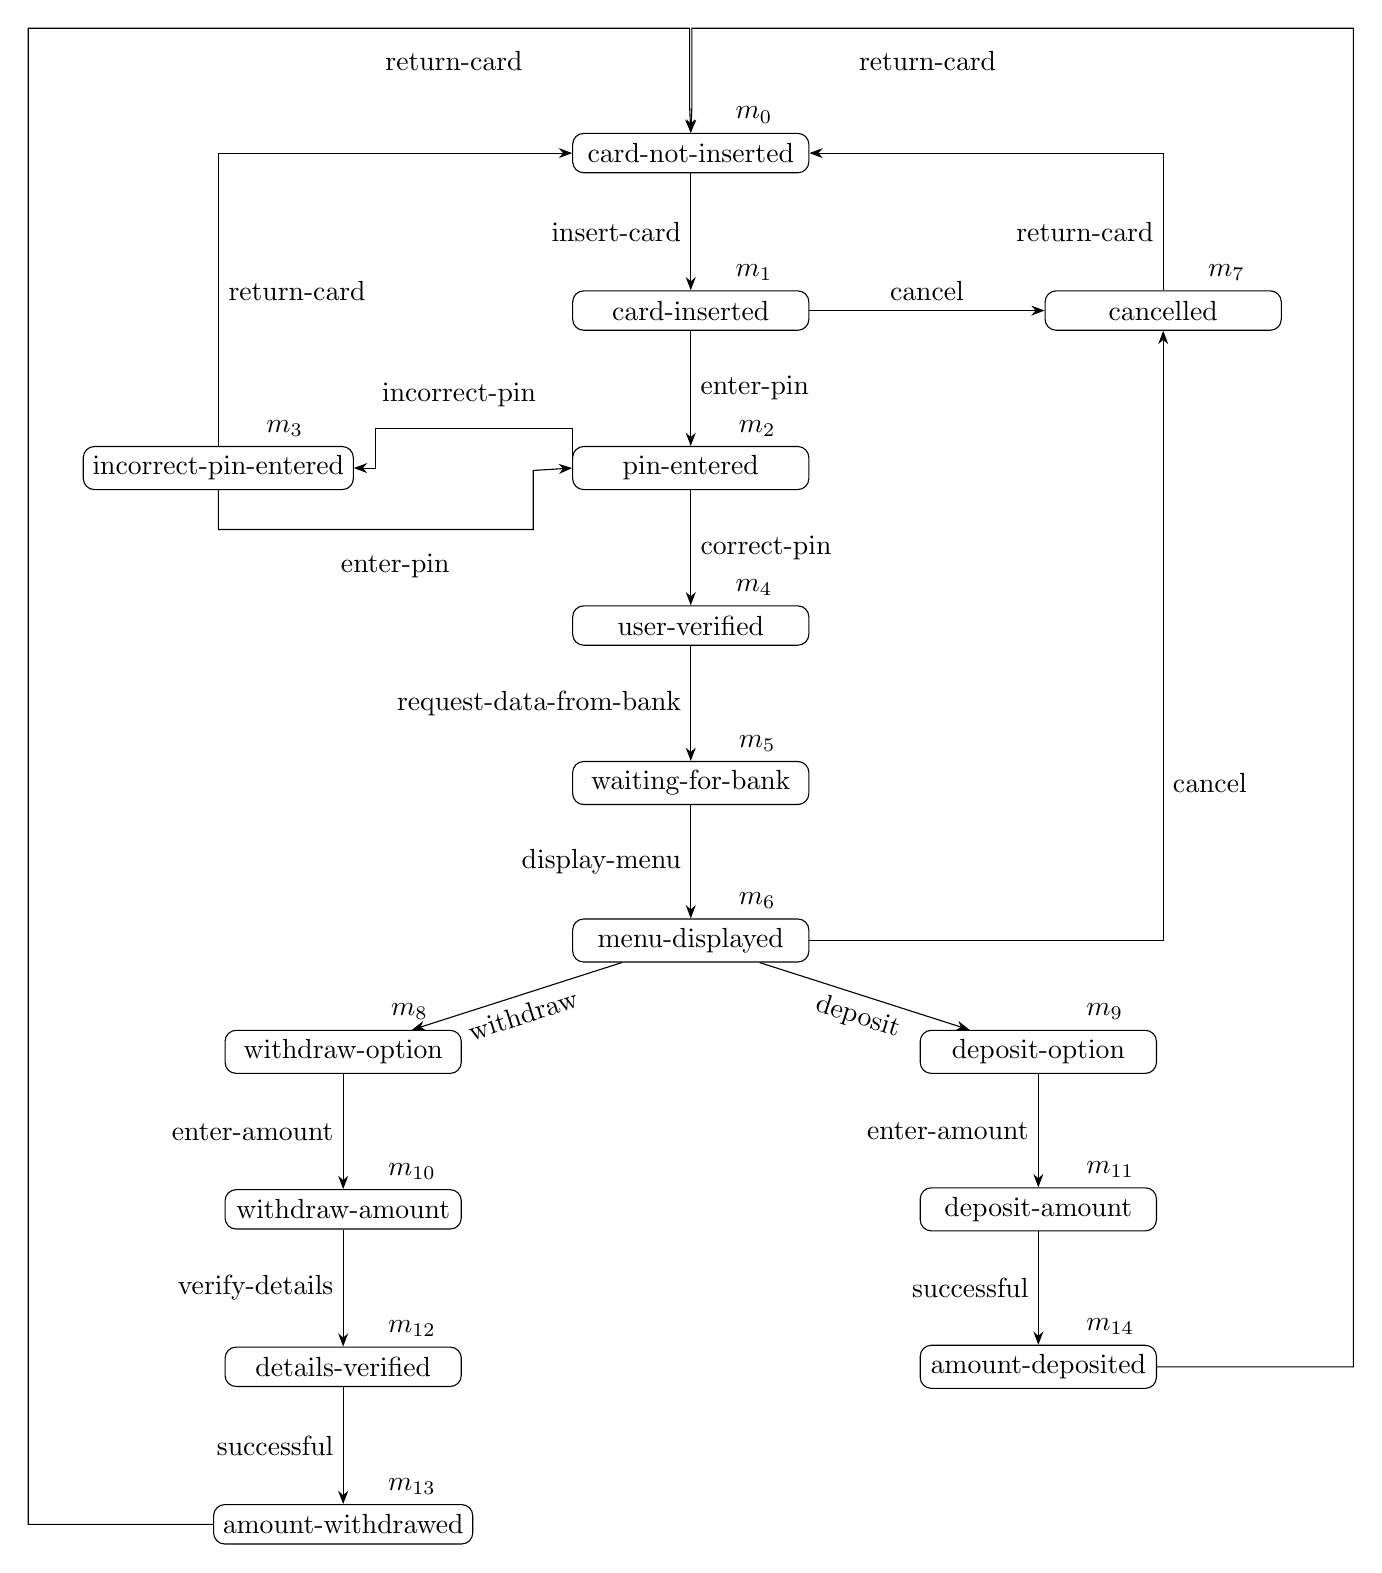
\begin{tikzpicture}[
		node distance=2cm,
		state/.style={rectangle, rounded corners, minimum width=3cm, minimum height=0.5cm,text centered, draw=black},
		process/.style={rectangle, minimum width=3cm, minimum height=0.5cm, text centered, draw=black, fill=orange!30},
		io/.style={trapezium, trapezium left angle=70, trapezium right angle=110, minimum width=3cm, minimum height=1cm, text centered, draw=black, fill=blue!30},
		decision/.style={diamond, minimum width=3cm, minimum height=1cm, text centered, draw=black, fill=green!30},
		]
		
		\node[state]       (m_0) [label={[label]30:$m_0$}]                                        {card-not-inserted};
		\node[state]         (m_1) [below of=m_0, label={[label]30:$m_1$}]                          {card-inserted};
		\node[state]         (m_2) [below of=m_1, label={[label]30:$m_2$}]                          {pin-entered};
		\node[state]         (m_3) [left of=m_2, xshift=-4cm, label={[label]30:$m_3$}]              {incorrect-pin-entered};
		\node[state]         (m_4) [below of=m_2, label={[label]30:$m_4$}]                          {user-verified};
		\node[state]         (m_5) [below of=m_4, label={[label]30:$m_5$}]                          {waiting-for-bank};
		\node[state]         (m_6) [below of=m_5, label={[label]30:$m_6$}]                          {menu-displayed};
		\node[state]         (m_7) [right of=m_1, xshift=4cm, label={[label]30:$m_7$}]              {cancelled};
		\node[state]         (m_8) [below left of=m_6, xshift=-3cm, label={[label]30:$m_8$}]        {withdraw-option};
		\node[state]         (m_9) [below right of=m_6, xshift=3cm, label={[label]30:$m_9$}]        {deposit-option};
		\node[state]         (m_10) [below of=m_8, label={[label]30:$m_{10}$}]                      {withdraw-amount};
		\node[state]         (m_11) [below of=m_9, label={[label]30:$m_{11}$}]                      {deposit-amount};
		\node[state]         (m_12) [below of=m_10, label={[label]30:$m_{12}$}]                     {details-verified};
		\node[state]         (m_13) [below of=m_12, label={[label]30:$m_{13}$}]                     {amount-withdrawed};
		\node[state]         (m_14) [below of=m_11, label={[label]30:$m_{14}$}]                     {amount-deposited};
		
		
		\draw [arrows=-Stealth] (m_0)                                                    --node[anchor=east]                                              {insert-card}        (m_1);
		\draw [arrows=-Stealth] (m_1)                                                    --node[anchor=west]                                              {enter-pin}         (m_2);
		\draw [arrows=-Stealth] (m_1)                                                    --node[anchor=south]                                             {cancel}       (m_7);
		\draw [arrows=-Stealth] (m_2.west) -- ++(0,0.5)  -- ++(-2.5,0) -- ++(0,-0.5)     --node[xshift=1.2cm,yshift=1.2cm,anchor=north,below]             {incorrect-pin}       (m_3.east);
		\draw [arrows=-Stealth] (m_3.south) -- ++(0,-0.5) -- ++(4,0) -- ++(0,0.75)       --node[xshift=-2cm,yshift=-1.5cm,anchor=south]                   {enter-pin}    (m_2.west);
		\draw [arrows=-Stealth] (m_3)                                                    |-node[xshift=1cm,yshift=-1.5cm,anchor=north,below]              {return-card} (m_0);
		\draw [arrows=-Stealth] (m_2)                                                    --node[anchor=west]                                              {correct-pin}       (m_4);
		\draw [arrows=-Stealth] (m_4)                                                    --node[anchor=east]                                              {request-data-from-bank}(m_5);
		\draw [arrows=-Stealth] (m_5)                                                    --node[anchor=east]                                              {display-menu}         (m_6);
		\draw [arrows=-Stealth] (m_6)                                                    -|node[yshift=2cm,anchor=west]                                              {cancel}       (m_7);
		\draw [arrows=-Stealth] (m_7)                                                    |-node[yshift=-1cm,anchor=east]                                              {return-card}    (m_0);
		\draw [arrows=-Stealth] (m_6)                                                    --node[anchor=north,sloped]                                      {withdraw} (m_8);
		\draw [arrows=-Stealth] (m_6)                                                    --node[anchor=north,sloped]                                      {deposit}       (m_9);
		\draw [arrows=-Stealth] (m_8)                                                    --node[anchor=east]                                              {enter-amount}        (m_10);
		\draw [arrows=-Stealth] (m_10)                                                   --node[anchor=east]                                              {verify-details}   (m_12);
		\draw [arrows=-Stealth] (m_12)                                                   --node[anchor=east]                                              {successful}       (m_13);
		\draw [arrows=-Stealth] (m_13) -- ++(-4,0) -- ++(0,19) -- ++(8.4,0) -- ++(0,-1)              --node[xshift=-3cm,yshift=0.5cm,anchor=south]                     {return-card}    (m_0.north);
		\draw [arrows=-Stealth] (m_9)                                                    --node[anchor=east]                                              {enter-amount} (m_11);
		\draw [arrows=-Stealth] (m_11)                                                   --node[anchor=east]                                              {successful}       (m_14);
		\draw [arrows=-Stealth] (m_14) -- ++(4,0) -- ++(0,17) -- ++(-8.4,0) -- ++(0,-1)               -- node[xshift=3cm,yshift=0.5cm,anchor=south]                                            {return-card} (m_0.north);
		
		\end{tikzpicture}
	\end{adjustbox}
		\caption{Mode graph of the ATM}
		\label{fig:Mode graph of the ATM}
\end{figure}
\end{frame}
\begin{frame}{Sample frame}
\end{frame}
\end{document}